\documentclass{standalone}
\usepackage{tikz-network}
\begin{document}
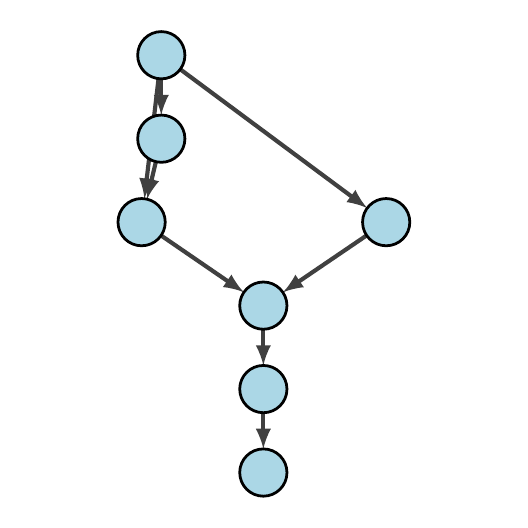
\begin{tikzpicture}
\clip (0,0) rectangle (6,6);
\Vertex[x=1.697,y=5.650]{LeastSquaresProblem1}
\Vertex[x=1.447,y=3.530]{VmecWrapper1}
\Vertex[x=2.993,y=2.470]{SurfaceRZFourier2}
\Vertex[x=2.993,y=1.410]{SpecBackoff1}
\Vertex[x=2.993,y=0.350]{NormalField1}
\Vertex[x=1.697,y=4.590]{QuasisymmetryRatioResidual1}
\Vertex[x=4.553,y=3.530]{TempOptimizable1}
\Edge[,Direct](LeastSquaresProblem1)(VmecWrapper1)
\Edge[,Direct](LeastSquaresProblem1)(QuasisymmetryRatioResidual1)
\Edge[,Direct](LeastSquaresProblem1)(TempOptimizable1)
\Edge[,Direct](VmecWrapper1)(SurfaceRZFourier2)
\Edge[,Direct](SurfaceRZFourier2)(SpecBackoff1)
\Edge[,Direct](SpecBackoff1)(NormalField1)
\Edge[,Direct](QuasisymmetryRatioResidual1)(VmecWrapper1)
\Edge[,Direct](TempOptimizable1)(SurfaceRZFourier2)
\end{tikzpicture}
\end{document}